%
% Шаблон для НИР версия 2021
%

\documentclass[a4paper,12pt]{article}


\usepackage{vkriate}
\usepackage{longtable}
\usepackage{multirow}


% Настройки для окружений с подчеркиваниями для подписей и пр.
\setFRMfontencoding{T2A}
\setFRMdfontencoding{T2A}
% thanks to A.Starikov
\setFRMfontfamily{cmr}
\setFRMdfontfamily{ptm}
\setFRMdfontsize{10pt}

% задает длину поля для подписи на титульной странице
\newFRMfield{xtitlesign}{32mm}

% поле для факультета или кафедры
\newFRMfield{fcath}{65mm}

%имя файла с библиографией в формате BibTex

\addbibresource{java.bib}

\begin{document}

% счетчики страниц, рисунков, таблиц
\regtotcounter{page}
\regtotcounter{figure}
\regtotcounter{table}

\renewcommand{\refname}{\centerline{СПИСОК ИСПОЛЬЗОВАННЫХ ИСТОЧНИКОВ}} 
\renewcommand{\contentsname}{\centerline{СОДЕРЖАНИЕ}} 
%\renewcommand{\refname}{Список источников}  % По умолчанию "Список литературы" (article)
%\renewcommand{\bibname}{Литература}  % По умолчанию "Литература" (book и report)

% титульная страница
\thispagestyle{empty}
\begin{center} \small
\textbf{МИНИСТЕРСТВО НАУКИ И ВЫСШЕГО ОБРАЗОВАНИЯ РОССИЙСКОЙ ФЕДЕРАЦИИ}\\
ФЕДЕРАЛЬНОЕ ГОСУДАРСТВЕННОЕ АВТОНОМНОЕ ОБРАЗОВАТЕЛЬНОЕ УЧРЕЖДЕНИЕ
ВЫСШЕГО  ОБРАЗОВАНИЯ\\
«Национальный исследовательский ядерный университет «МИФИ»\\
\textbf{Обнинский институт атомной энергетики} – \\
филиал федерального государственного автономного образовательного учреждения высшего\\
образования «Национальный исследовательский ядерный университет «МИФИ»\\
(ИАТЭ НИЯУ МИФИ)
\end{center}
%\vfill
\medskip

% Направление подготовки следует уточнять,
% магистры и бакалавры могут иметь разные наименования
\begin{center}
\begin{tabular}{rl}
Отделение & \useFRMfield{fcath}[\large Интеллектуальные кибернетические системы] \\ 
Направление подготовки & \useFRMfield{fcath}[\large Информационные системы и технологии] \\ 
\end{tabular} 
\end{center}

\vfill

\large 

\begin{center}
	Научно-исследовательская работа \\
	
	\medskip
	
	\textbf{\Large 
		Java приложение для выбора параметров анализа и визуализации расчётных данных
	}
	
\end{center}

\vspace{1cm}

\begin{tabular*}{\textwidth}{lcr}
Студент группы ИС-Б18 & \useFRMfield{xtitlesign} & Михайлова А.В.\\
& & \\
Руководитель & & \\
к.т.н., доцент отд. ИКС & \useFRMfield{xtitlesign} & Мирзеабасов О.А.
\end{tabular*}


\vfill
\large

\begin{center}
Обнинск, 2022 г
\end{center}

\onehalfspacing

\pagebreak

% реферат
\thispagestyle{empty}

\section*{\centering РЕФЕРАТ}

% возможно, кол-во источников придется вставлять вручную
Работа \total{page} стр., \total{figure} рис. , \totalmycitecounts ист. 

ЯЗЫК ПРОГРАММИРОВАНИЯ JAVA, ОБРАБОТКА ДАННЫХ, РАСЧЁТНЫЕ ПРОГРАММЫ, ВИЗУАЛИЗАЦИЯ, НАТРИЕВЫЙ КОНТУР, ГРАФИЧЕСКИЙ ИНТЕРФЕЙС

Работа посвящена проектированию и разработке приложения на языке Java с графичсеким интерфейсом, которое позволит задавать параметры для последующей визуализации расчетных данных.

Разработанная программа автоматизирует ручную обработку данных и позволит избежать ошибок при последующей визуализации.

%\pagebreak
%\thispagestyle{empty}
%
%\section*{\centering ОПРЕДЕЛЕНИЯ}
%
%Репозиторий --- место, где хранятся и поддерживаются версии каких-либо данных. 
%
%\pagebreak
%
%\section*{\centering ОБОЗНАЧЕНИЯ И СОКРАЩЕНИЯ}
%
%
%НИР --- Научно-исследовательская работа
%
%СПВ --- Система поддержки версий
%


\pagebreak

% титульная страница - номер 1, остальные страницы до Содержания не нумеруются
\tocloftpagestyle{empty}

\tableofcontents
% если нужно добавить "Стр." над номерами страниц - раскомментируйте следующую команду
%\addtocontents{toc}{~\hfill\textbf{Стр.}\par}

\pagebreak

\setcounter{page}{3}

\section*{\centering ВВЕДЕНИЕ}
\addcontentsline{toc}{section}{ВВЕДЕНИЕ}
% введение

Анализ данных – это комплекс методов и приложений, связанных с алгоритмами обработки данных и не имеющих четко фиксированного ответа на каждый поступающий объект. Это будет выделять их от классических алгоритмов, например реализующих сортировку или словарь. Статистическая обработка данных и визуализация результатов анализа — это неизбежный шаг работы с данными, полученными в различных областях естественных наук, в социологии, психологии или экономике.

Необходимым условием современного статистического анализа данных является эффективное использование компьютерных программ, от функциональной полноты и алгоритмической продуманности которых зависит итоговая интерпретация результатов исследования и надежность выводов. 

Вычислительные программы, используемые для моделирования сложных физических процессов, зачастую имеют значительное количество настроечных параметров и условий выполнения расчетов. Это относится и к программе blleak16d, параметры которой хранятся в текстовых файлах и редактируются непосредственно в них. Помимо конфигурационных файлов, существуют так же расчетные файлы, содержащие информацию об итогах расчета вычислительной программы. Такие файлы перенасыщенны информацией причем очень часто повторяющейся, что усложняет процесс анализа. Чтобы сделать грамотный анализ расчётных данных и их визуализацию, нужно выбрать различные параметры и переменные для отображения. С учётом объёма информации в файлах, сделать это рациональнее с помощью компьютерной программы с графическим интерфейсом.  


Целью данной научно-исследовательской работы является разработка Java-приложения с графическим интерфейсом для задания параметров визуализации. 
\medskip

В ходе выполнения работы необходимо решить следующие задачи:

\begin{itemize}
	\item выполнить анализ структуры конфигурационных и расчётных файлов;
	\item разработать вспомогательные классы для считывания конфигурации;
	\item разработать классы, описывабщие структуру расчетных файлов;
	\item спроектировать и разработать пользовательский интерфейс задания параметров расчётных данных.	
\end{itemize} % текст введения в файле intro.tex
\pagebreak

%\input{Post_zad}
\pagebreak
% первая часть

\section{Структура и составляющие вычислительной модели контура}

\subsection{Обзор предметной области}

В структуре крупномасштабной атомной отрасли будущего, перспективным направлением развития ядерной энергетики без использования атомных электростанций является создание и эксплуатация реакторов на быстрых нейтронах.

Реактор на быстрых нейтронах позволяет превращать отработавшее ядерное топливо в новое топливо для АЭС, образуя замкнутый цикл использования ядерного топлива, и позволяя вместо доступных ныне 3\%, использовать около 30\% потенциала ядерного топлива, что обеспечит перспективу ядерной энергетике на тысячелетия.

По сравнению с распространенным реактором на тепловых нейтронах, реакторы на быстрых нейтронах обладают рядом достоинств с точки зрения безопасности: в реакторе нет высокого давления, в них практически нет риска потери теплоносителя по причине выкипания, нет риска пароциркониевой реакции, ставшей одной из причин взрывов на Фукусимской АЭС. С другой стороны, популярный теплоноситель натрий бурно реагирует с водой и горит на воздухе, что усложняет любую аварию с утечкой теплоносителя.

В реакторах с натриевым теплоносителем мы не можем использовать двухконтурную схему, где первый контур заполнен натрием, а второй — водой, поскольку случайное взаимодействие облученного натрия с водой приведет к особо тяжелым последствиям (рисунок~\ref{fig:bn}). В ходе реакции этих двух веществ выделяется взрывоопасный водород, и в случае взрыва нейтрализовать фонящий натрий будет крайне проблематично. Поэтому используют трехконтурную схему. Первый контур — натриевый (на рисунке он показан красным в центре реактора), потом теплообменник и еще один (промежуточный) натриевый контур (желтый цвет), позволяющий снизить степень облучения натрия, и только в третьем контуре используется вода, установлена турбина, тепловые части и остальное оборудование. Три контура усложняют как эксплуатацию реактора, так и управление им.

\begin{figure}[H]
	\centering
	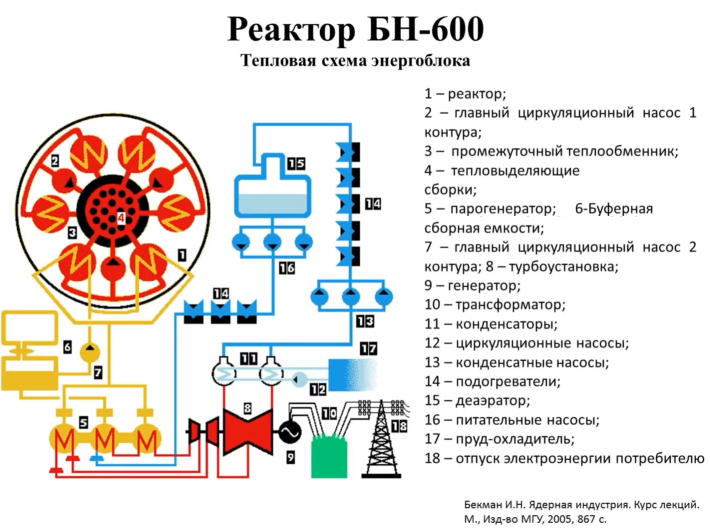
\includegraphics[width=1\linewidth]{pics/bn}
	\caption{Схема энергоблока реактора на быстрых нейтронах}
	\label{fig:bn}
\end{figure}

Высокая химическая активность натрия порождает ряд специфических проблем. Изучение возможных последствий подобных аварий, их моделирование, а также запуск всевозможных расчетов являются важным направлением анализа безопасности установок с натриевым теплоносителем. С этой целью была разработана программа моделирования, визуализации результатов расчетов и настройки компонентов гидродинамики многокомпонентной смеси blleak16d.

Вычислительные программы, используемые для моделирования сложных физических процессов, в том числе и blleak16d, имеют большое количество различных конфигурационных и выходных файлов, которые в свою очередь содержат значительное количество разнообразной информации. 

Каждый файл конфигурации имеет сложную структуру. Один файл может содержать ссылки на несколько других и так далее. В свою очередь, в файлах содержится много однотипной и повторяющейся информации. Это значительно усложняет процесс анализа данных, если проводить его вручную.
Для облегчения анализа данных, имеет смысл провести визуализацию, которая позволит наглядно увидеть переломные моменты моделирования, т.е. моменты, в которых произошла моделируемая авария. 

Для визуализации, требуется сначала выбрать определенные параметры и переменные для вывода. Сделать это вручную, опять же, было бы очень проблематично из-за сложной иерархии файлов и большого объёма данных. Целью данной научно-исследовательской работы как раз выступает создания приложения с графическим интерфейсом, которое бы облегчило процесс подготовки к визуализации. А в последующем, могло бы и проводить саму визуализацию расчетных данных. 



\subsection{Структура конфигурационных и выходных вычислительных файлов}

Перед тем, как приступить к написанию пользовательского приложение, надо проанализировать структуру файлов, с которыми будет работать это приложение. 

В качестве основных файлов, который задают параметры контура, можно выделить:
\begin{itemize}
\item mainconf.txt – этот файл содержит в себе базовые параметры для всей системы и названия основных конфигурационных файлов, в которые входят файлы с параметрами узлов, каналов и временного сценария;
\item bounds.txt – этот файл включает в себя информацию о количестве узлов и список всех узлов системы со ссылкой на конфигурационный файл для каждого узла;
\item timescen.txt – этот файл хранит данные временного сценария процесса моделирования;
\item chanprof.txt – этот файл содержит в себе информацию о каналах, их количестве и геометрии каждого канала, а также хранит ссылки на файлы конфигурации каналов.
\end{itemize}

Все файлы представляют собой сложную структуру, т.к. помимо описания общей информации они содержат названия других файлов, содержимое которых, в свою очередь, является также немаловажным.

Основная информация, используемая для анализа, хранится в файлах с описанием узлов, каналов, геометрии и т.д. Все данные в этих файлах хранятся в виде таблиц с заданной структурой. Каждый такой файл представляет собой массивную таблицу данных без названия полей и четкой границы столбцов. 

Кроме конфигурационных файлов, в ходе работы вычислительной программы появляются выходные расчётные файлы. Основным их содержимым являются численные данные, записанные по столбцам, которые представляют собой основную расчётную информацию и результаты снятия показаний в контуре во время протекания реакции. Сложность анализа таких данных заключается в том, что столбцы файла не имеют названий, а разделителем данных по столбца является символ пробела. Учитывая, что один такой файл имеет очень большой объём информации, выбор данных пользователем напрямую является нерезультативным и отнимает много времени. 


Чтобы более наглядно представить структуру конфигурационных и выходных вычислительных файлов, можно посмотреть на рисунок~\ref{fig:scheme}, на которой представлена иерархия этих файлов. 

\begin{figure}[H]
	\centering
	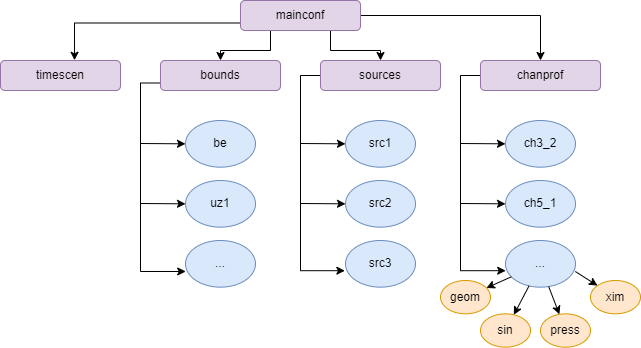
\includegraphics[width=1\linewidth]{pics/scheme}
	\caption{Иерархическая структура файлов}
	\label{fig:scheme}
\end{figure}

По вышеперечисленным причинам, необходимо разработать приложение, которое сможет считывать и обрабатывать файлы такого рода и предоставлять информацию в удобном для пользователя формате, для того, чтобы потом легко выбрать нужные параметры для визуализации. 


  % первая глава - в файле part1.tex
\pagebreak
% первая часть

\section{Программный язык и среда разработки}

\subsection{Java}

На сегодняшний момент язык Java является одним из самых распространенных и популярных языков программирования. Первая версия языка появилась еще в 1996 году в недрах компании Sun Microsystems, впоследствии поглощенной компанией Oracle. Java задумывался как универсальный язык программирования, который можно применять для различного рода задач. И к настоящему времени язык Java проделал большой путь, было издано множество различных версий. Текущей версией является Java 18, которая вышла 22 марта 2022 года. А Java превратилась из просто универсального языка в целую платформу и экосистему, которая объединяет различные технологии, используемые для целого ряда задач: от создания десктопных приложений до написания крупных веб-порталов и сервисов. Кроме того, язык Java активно применяется для создания программного обеспечения для множества устройств: обычных ПК, планшетов, смартфонов и мобильных телефонов и даже бытовой техники. Достаточно вспомнить популярность мобильной ОС Android, большинство программ для которой пишутся именно на Java.

\subsubsection{Язык Java}

Ключевой особенностью языка Java является то, что его код сначала транслируется в специальный байт-код, независимый от платформы. А затем этот байт-код выполняется виртуальной машиной JVM (Java Virtual Machine). В этом плане Java отличается от стандартных интерпретируемых языков как PHP или Perl, код которых сразу же выполняется интерпретатором. В то же время Java не является и чисто компилируемым языком, как С или С++.

Подобная архитектура обеспечивает кроссплатформенность и аппаратную переносимость программ на Java, благодаря чему подобные программы без перекомпиляции могут выполняться на различных платформах - Windows, Linux, Mac OS и т.д. Для каждой из платформ может быть своя реализация виртуальной машины JVM, но каждая из них может выполнять один и тот же код.

Java является языком с Си-подобным синтаксисом и близок в этом отношении к C/C++ и C\#. Поэтому, если вы знакомы с одним из этих языков, то овладеть Java будет легче.

Еще одной ключевой особенностью Java является то, что она поддерживает автоматическую сборку мусора. А это значит, что вам не надо освобождать вручную память от ранее использовавшихся объектов, как в С++, так как сборщик мусора это сделает автоматически за вас.

Java является объектно-ориентированным языком. Он поддерживает полиморфизм, наследование, статическую типизацию. Объектно-ориентированный подход позволяет решить задачи по построению крупных, но в тоже время гибких, масштабируемых и расширяемых приложений.

По данным компании Oracle, программы на Java запускаются на 3 млрд девайсов. Это маркетинговое сообщение сложно проверить. Тем не менее Java широко используется и входит в число самых востребованных языков, это не вызывает сомнения.

Например, подавляющее большинство крупных компаний так или иначе используют Java. Очень много серверных приложений для корпораций написаны на этом языке. Например, речь идёт о программах для финансовых организаций, которые обеспечивают проведение транзакций, фиксацию торговых операций.

На Java написано много веб-приложений. Популярные фреймворки, в том числе Spring, Stuts, JSP, используются для создания разных приложений в вебе: от ecommerce-проектов до крупных порталов, от образовательных платформ до правительственных ресурсов.

Мобильная разработка — ещё одна область использования Java. На этом языке пишут приложения для устройств, работающих под управлением ОС Android.

На Java создают клиентские приложения. Простой и близкий разработчикам пример: IDE NetBeans написано на «джаве».

Также Java применяется для работы с Big Data, разработки программ для научных целей, например, обработки естественных языков, программирования приборов — от бытовых девайсов до промышленных установок.

То есть на Java можно писать разные типы приложений: веб, мобильный и десктопный софт, игры и так далее. Традиционно у этого языка сильные позиции в промышленном программировании, в сегменте крупных компаний (т.н. энтерпрайз).

Java — достаточно распространённый язык: им пользуется большое количество разработчиков, и решение практически любой проблемы, которая может возникнуть при работе с Java, уже кто-то придумал. Благодаря тысячам библиотек и форумов, можно найти готовое решение почти в любой ситуации. На GitHub, например, есть открытые проекты и документация, а на форуме Stack Overflow можно обратиться за помощью к комьюнити.

Язык Java строго типизирован. То есть любая переменная или выражение имеет определённый тип уже на момент компиляции, что упрощает выявление каких-либо проблем. Компилятор сам подсказывает программисту, где тот допускает ошибку, и не даёт её совершить.

Все библиотеки, написанные когда-либо для Java, — это классы, которые отвечают за функциональность языка. Любое приложение на Java — набор классов, описывающих разные объекты. Это хорошо, потому что позволяет создавать сложные программы, но простые в поддержке. И в целом Java — мультипарадигменный язык, то есть поддерживает множество принципов программирования, что позволяет эффективно решать разные задачи.


\subsubsection{Графический интерфейс в Java}

GUI (графический интерфейс пользователя) в Java — это простой в использовании конструктор визуального восприятия для Java-приложений. Он состоит в основном из графических компонентов, таких как кнопки, ярлыки, окна и т.д., с помощью которых пользователь может взаимодействовать с приложением. GUI играет важную роль в создании простых интерфейсов для Java-приложений.

Графический интерфейс в Java прошел весьма тернистый путь развития и становления. Долгое время его обвиняли в медленной работе, жадности к ресурсам системы и ограниченной функциональности.

Первой попыткой Sun создать графический интерфейс для Java была библиотека AWT (Abstract Window Toolkit) — инструментарий для работы с различными оконными средами. Sun сделал прослойку на Java, которая вызывает методы из библиотек, написанных на С. Библиотечные методы AWT создают и используют графические компоненты операционной среды. С одной стороны, это хорошо, так как программа на Java похожа на остальные программы в рамках одной ОС. Но при запуске ее на другой платформе могут возникнуть различия в размерах компонентов и шрифтов, которые будут портить внешний вид программы.

Чтобы обеспечить мультиплатформенность AWT интерфейсы вызовов компонентов были унифицированы, вследствие чего их функциональность получилась немного урезанной. Да и набор компонентов получился довольно небольшой. Так, например, в AWT нет таблиц, а в кнопках не поддерживается отображение иконок. Тем не менее, пакет java.awt входит в Java с самого первого выпуска и его можно использовать для создания графических интерфейсов.

Таким образом, компоненты AWT не выполняют никакой "работы". Это просто «Java-оболочка» для элементов управления той операционной системы, на которой они работают. Все запросы к этим компонентам перенаправляются к операционной системе, которая и выполняет всю работу.

Использованные ресурсы AWT старается освобождать автоматически. Это немного усложняет архитектуру и влияет на производительность. Написать что-то серьезное с использованием AWT будет несколько затруднительно. Сейчас ее используют разве что для апплетов.

Вслед за AWT Sun разработала графическую библиотеку компонентов Swing, полностью написанную на Java. Для отрисовки используется 2D, что принесло с собой сразу несколько преимуществ. Набор стандартных компонентов значительно превосходит AWT по разнообразию и функциональности. Swing позволяет легко создавать новые компоненты, наследуясь от существующих, и поддерживает различные стили и скины.

Создатели новой библиотеки пользовательского интерфейса Swing не стали «изобретать велосипед» и в качестве основы для своей библиотеки выбрали AWT. Конечно, речь не шла об использовании конкретных тяжеловесных компонентов AWT (представленных классами Button, Label и им подобными). Нужную степень гибкости и управляемости обеспечивали только легковесные компоненты. На диаграмме наследования (рисунок~\ref{fig:swing-base}) представлена связь между AWT и Swing.

\begin{figure}[H]
	\centering
	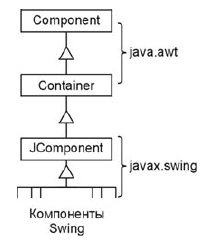
\includegraphics[width=0.5\linewidth]{pics/swing-base}
	\caption{Диаграмма наследования}
	\label{fig:swing-base}
\end{figure}



Важнейшим отличием Swing от AWT является то, что компоненты Swing вообще не связаны с операционной системой и поэтому гораздо более стабильны и быстры. Такие компоненты в Java называются легковесными (lightweight), и понимание основных принципов их работы во многом объяснит работу Swing.

Чтобы понять разницу между AWT и Swing, надо посмотреть на рисунок~\ref{fig:AWT-Swing-diff}.


\begin{figure}[H]
	\centering
	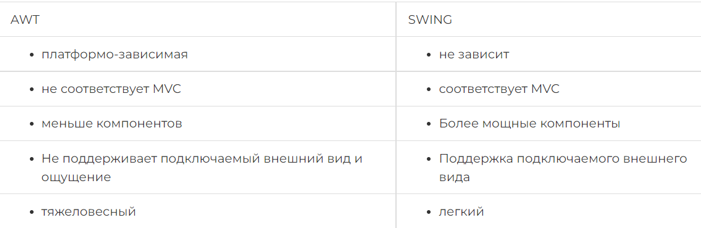
\includegraphics[width=1\linewidth]{pics/AWT-Swing-diff}
	\caption{AWT и Swing}
	\label{fig:AWT-Swing-diff}
\end{figure}

Компонент Swing следует архитектуре Model-View-Controller для выполнения следующих критериев:
\begin{itemize}
\item Одного API должно быть достаточно для поддержки множественного внешнего вида;
\item API должен быть ориентирован на модель, чтобы не требовалось, чтобы у API самого высокого уровня были данные;
\item API заключается в использовании модели Java Bean, чтобы инструменты Builder и IDE могли предоставлять разработчикам более качественные сервисы для использования.
\end{itemize}

Иерархия классов в Swing представлена на рисунке~\ref{fig:hierarchy}.
\begin{figure}[H]
	\centering
	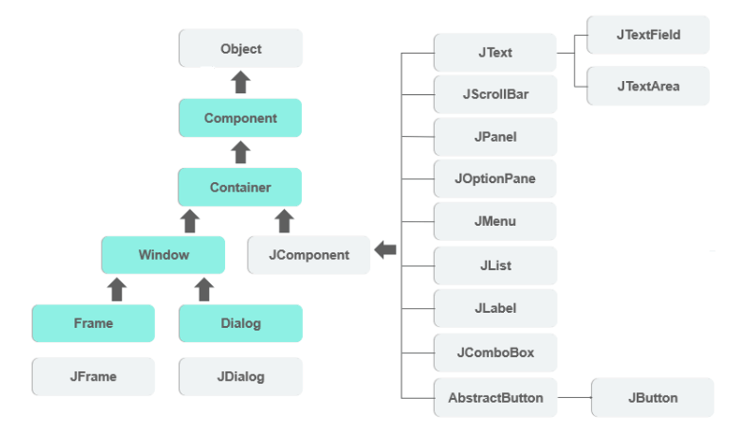
\includegraphics[width=1\linewidth]{pics/hierarchy}
	\caption{Иерархия классов Swing}
	\label{fig:hierarchy}
\end{figure}


Все компоненты в свинге, такие как JButton, JComboBox, JList, JLabel, унаследованы от класса JComponent, который можно добавить в классы контейнера.

Контейнеры – это окна, такие как рамка и диалоговые окна. Основные компоненты являются строительными блоками любого графического приложения. Такие методы, как setLayout, переопределяют макет по умолчанию в каждом контейнере. Контейнеры, такие как JFrame и JDialog, могут добавлять только компонент к себе.

\subsection{Среда разработки NetBeans}

NetBeans IDE - бесплатная интегрированная среда разработки с открытым исходным кодом для разработчиков программного обеспечения. Среда предоставляет все средства, необходимые для создания профессиональных десктоп приложений, корпоративных, мобильных и веб-приложений на платформе Java, а также C/C++, PHP, JavaScript, Groovy и Ruby. 
Основные характеристики NetBeans IDE:


\begin{itemize}
\item рабочая область среды IDE является полностью настраиваемой - существует возможность пользовательской настройки действий, выполняемых с помощью панели, назначения "горячих" клавиш и т.д.;
\item IDE имеет в своем составе расширенный многоязыковой редактор для различных языков программирования - Java, C/C++, Ruby, Groovy, PHP, JavaScript, CSS, XML, HTML, RHTML, JSP, документацию Javadoc. Существует возможность расширения функций редактора с целью поддержки любого другого языка;
\item производится проверка ошибок во время ввода, отображение вариантов для автозавершения кода и фрагментов документации по требуемому языку программирования;
\item редактор может генерировать и вставлять в исходный код стандартные фрагменты кода на Java или других языках;
\item браузер классов позволяет просматривать иерархию и структуру любого класса Java - отображаются интерфейсы, базовые классы, производные классы и члены классов;
\item существует возможность перемещения любой вкладки редактора в пределах рабочего пространства IDE и за её пределы, создавая независимое окно, которое можно переместить на второй экран;
\item возможность группирования связанных проектов - создавая группы проектов, можно быстро открывать и закрывать несколько сгруппированных проектов одновременно;
\item расширенные средства для выполнения контекстно-зависимого поиска по всей среде IDE, справочным материалам и всем открытым проектам и файлам;
\item существует возможность создания проектов в свободном формате или начинать работу с проектом с шаблона. В комплекте со средой IDE поставляются шаблоны и примеры проектов для приложений Java SE, мобильных, веб-приложений и приложений уровня предприятия, приложений JavaFX, подключаемых модулей NetBeans, приложений Groovy, PHP, C/C++, Ruby и Ruby on Rails;
\item NetBeans IDE является платформой для построения десктоп приложений с функциональным пользовательским интерфейсом, т.к. представляет из себя фреймворк к Java библиотеке Swing;
\item NetBeans имеет встроенную поддержку CVS, Mercurial и Subversion. Для просмотра изменений используется редактор с цветовыми обозначениями.
\end{itemize}

Возможности программирования в NetBeans:
\begin{itemize}
\item разработка Java десктоп приложений с профессиональными графическими интерфейсами пользователя. Используется визуальный редактор - Swing GUI Builder. Работа осуществляется путем перетаскивания элементов графического интерфейса из палитры на холст. Предварительное позиционирование элементов можно осуществлять с помощью указателя мыши. Панель свойств и инспектор компонентов предоставляют возможность тонкой настройки каждого компонента интерфейса; 
\item создание веб-приложений и корпоративных приложений в соответствии со стандартами. Среда NetBeans предоставляет полную поддержку Java EE 6. Позволяет разрабатывать веб-страницы, сервлеты, веб-сервисы, Enterprise Java Beans (EJB), проекты Java EE с использованием JavaServer Faces 2.0 (Facelets), Spring, Struts и Hibernate;
\item программирование на PHP, поддержка всех сопутствующих языков программирования, технологий и веб-стандартов. Возможность создавать проекты PHP на основе платформы Zend или Symfony. Редактор PHP динамически интегрирован с функциями редактирования HTML, JavaScript и CSS. Проекты PHP могут быть развёрнуты из среды NetBeans на локальном или удаленном сервере при взаимодействии через FTP или SFTP;
\item возможность создания, тестирования, отладки и внедрения приложений, функционирующих на мобильных телефонах, карманных компьютерах, телеприставках и встраиваемых системах. Visual Mobile Designer (VMD) создает всю необходимую модульную инфраструктуру проекта и обеспечивает быструю разработку графических интерфейсов путём перетаскивания в рабочую область компонентов - экран ожидания, экран входа в систему, обозреватель файлов, средство составления сообщений SMS и экран заставки. Возможность создания пользовательского интерфейса на основе SVG;
\item использование JavaFX Composer для визуального структурирования приложения JavaFX с графическим интерфейсом, аналогично конструктору GUI Swing для Java десктоп приложений;
\item возможность разработки профессиональных приложений на языках C, C++ для различных платформ - Windows, Linux, Mac и Solaris. Поддерживаются все широко используемые компиляторы - GNU, Cygwin и MinGW. Существует возможность установки требуемого компилятора, определений препроцессора, параметров времени компиляции и т.д.;
\item расширенные возможности по работе с базами данных - встроенный клиент к базам данных - MySQL, Postgres, Oracle и др., редактор запросов SQL, возможность редактировать таблицы баз данных напрямую через редактор таблиц;
\item интеграция с серверами приложений и контейнерами сервлетов - автоматическое развёртывание приложений, управление сервером - запуск, остановка, перезапуск;
\item многоязычный пользовательский интерфейс с поддержкой русского языка;
\item расширение функциональности с помощью подключаемых модулей, гибкая система управления компонентами, модулями, обновление и загрузка модулей через интернет.

\end{itemize}

NetBeans - единственная IDE, которая устроит и начинающего разработчика и профессионала. Наличие подробной встроенной справочной системы обеспечит быстрый старт для начинающих пользователей.

 % вторая глава - в файле part2.tex
\pagebreak
% вторая часть

\section{Проектирование и разработка приложения для задания параметров}

\subsection{Разработка вспомогательных классов}

Первоначальным этапом разработки было создание вспомогательных классов для работы с исходными данными.

Некоторые операции, которые являются общими для нескольких классов, могут быть перенесены на вспомогательные классы, которые затем используются с помощью композиции объекта. 

Каждый отдельный класс относится к конкретному типу файла. Для всех файлов мы можем выделить один общий метод – это чтение информации из файла. Чтобы не повторять в каждом классе эту операцию, можно воспользоваться одним из ключевых понятий объекто-ориентированного программирования, а именно – наследованием. 

Наследование является неотъемлемой частью Java. При использовании наследования вы говорите: этот новый класс похож на тот старый класс. В коде это пишется как extends, после которого указываете имя базового класса. Тем самым вы получаете доступ ко всем полям и методам базового класса. Используя наследование, можно создать общий класс, которые определяет характеристики, общие для набора связанных элементов. Затем вы можете наследоваться от него и создать новый класс, который будет иметь свои уникальные характеристики. Главный наследуемый класс в Java называют суперклассом. Наследующий класс называют подклассом. Получается, что подкласс — это специализированная версия суперкласса, которая наследует все члены суперкласса и добавляет свои собственные уникальные элементы.

Исходный код суперкласса приведён в приложении в листинге~\ref{DefReader}.

От этого суперкласса были наследованы все остальные подклассы, которые реализуют работу с каждым типом файлов. 

В основном, эти подклассы включают в себя методы, которые проводят синтаксический анализ (парсинг) полученного ранее текста файла. Затем, полученная в результате этой операции информация присваивается полям класса. Таким образом, текст файла структурируется по полям класса. 

Для корректного парсинга и выделения подстрок в программе использовались регулярные выражения. Функция setChans (листинг~\ref{list-1}) является примером реализации метода синтаксического анализа текста. 

\begin{Program}
	\begin{MyCode}
		private void setChans(){
			if (fileInf == null) {
				System.out.println("Error");
			} else {
				
				
				for (int i = 1; i <= n*2; i++) {
					String[] split = fileInf.get(i).trim().split("\\s+");
					if((split.length == 2) && (Integer.valueOf(split[1]) == 1)) {
						
						String[] split1 = fileInf.get(i+1).trim().split("\\s+");
						ChanProf ch = new ChanProf(Integer.valueOf(split[0]), Integer.valueOf(split1[0]), Integer.valueOf(split1[1]), split1[2]);
						chans.add(ch);
						
					}
					i++;
					
				}
			}
		}
			
		\end{MyCode}
		\caption{Обработка и синтаксический анализ текста}\label{list-1}
	\end{Program}


При анализе текста исходных файлов можно заметить, что в некоторых файлах имеются повторяющиеся строки с одинаковой структурой. Целесообразно выделить их в отдельные классы. Такие классы представляют собой структуры для хранения информации. Основные методы таких классов – это set- и get-методы.

Также, в отдельную группы можно выделить классы, которые работают с файлами, которые используются для сохранения результатов моделирования определенного канала. Структура таких фалов может меняться: некоторые столбцы могут добавляться или наоборот убраться. Поэтому, было решено выделить структуру этих файлов в отдельный файл с метаданными по столбцам. 

Пример такого файла представлен на рисунке~\ref{fig:meta}.
\begin{figure}[H]
	\centering
	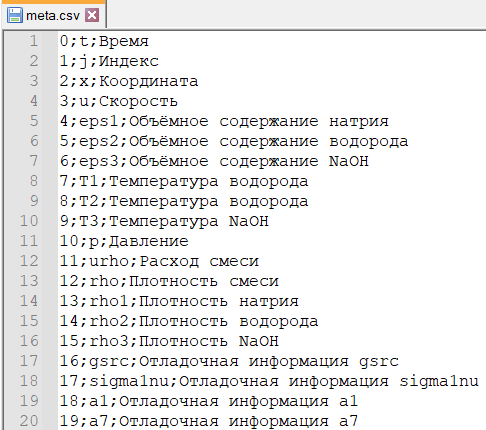
\includegraphics[width=0.7\linewidth]{pics/meta}
	\caption{Структура файла CSV}
	\label{fig:meta}
\end{figure}

Он представляет собой CSV-файл. В качестве разделителя здесь выступает точка с запятой. Первый столбец – это индекс столбца в файле с результатами моделирования канала. Второй столбец – это идентификатор переменной, который используется в выходном файле канала. Третий столбец – это полное название переменной. Оно нужно для последующего отображения в программе, чтобы пользователь мог выбрать конкретные физическое величины, а не идентификаторы. 

Для работы с файлом SCV и файлом с результатами моделирования канала было написано три класса: ChanCol, ChanFile и ChanInTime.

Класс ChanCol реализует колонку выходного файла с результатами. Поля этого класса полностью совпадают со структурой файла CSV. 

Исключение составляет лишь поле, в котором записан путь к файлу с данными по умолчанию. Так как CSV файла с метаданными по столбцам может попросту не быть, то было решено «вшить» в программу файл по умолчанию, в котором записана информация по колонкам, которая актуальна на данный момент. 

Также, момент с отсутствием файла с метаданными был учтён и в коде программы (листинг~\ref{list-2}).

\begin{Program}
	\begin{MyCode}
		try {
			br = new BufferedReader(new FileReader(path));
			while ((line = br.readLine()) != null) {
				String[] data = line.split(";");
				ChanCol chanCol = new ChanCol(Integer.valueOf(data[0]), data[1], data[2]);
				arr.add(chanCol);
				
			}
			
			
		} catch (FileNotFoundException ex) {
						
			try {
				br = new BufferedReader(new FileReader(ChanCol.defaultCSV));
				while ((line = br.readLine()) != null) {
					String[] data = line.split(";");
					ChanCol chanCol = new ChanCol(Integer.valueOf(data[0]), data[1], data[2]);
					arr.add(chanCol);
					
				}
				
			} catch (FileNotFoundException ex1) {
				Logger.getLogger(ChanCol.class.getName()).log(Level.SEVERE, null, ex1);
			} catch (IOException ex1) {
				Logger.getLogger(ChanCol.class.getName()).log(Level.SEVERE, null, ex1);
			}
		
	\end{MyCode}
	\caption{Обработка FileNotFoundException}\label{list-2}
\end{Program}

В вышеприведенном участке кода реализуется парсинг данных из файла CSV. В блоке catch (FileNotFoundException ex) производится обработка исключения FileNotFoundException. Если файл не найден, то для дальнейшей работы используется файл по умолчанию, упомянутый выше. 

Класс ChanInTime представляет состояния канала в заданный момент времени. В качестве полей класса выступают такие значения, как время, список переменных (массив объектов класса ChanCol) и список массивов значений столбцов. Объект такого класса представляет собой строки выходного файла, которые соответствуют заданному моменту времени. Т.е. мы имеем один момент времени и несколько точек, которым соответствуют значения из файла с результатами моделирования.

Класс ChanFile представляет данные из расчетного файла в виде массива (списка) состояний в каждый момент времени. Здесь используется описанный выше класс ChanInTime. Массив из объектов этого класса будет описывать все моменты времени моделирования. Таким образом, объект класса ChanFile будет содержать в себе полную информацию выходного файла с результатами моделирования.

\subsection{Разработка пользовательского интерфейса}

Приложение представляет собой программу, написанную на языке Java с использованием технологии Swing. Графический интерфейс позволяет удобно и интуитивно работать с программой. Приложение облегчает работу пользователя, т.к. проводит выборку необходимых параметров для визуализации автоматически. 
Программа представляет собой приложение с графическим интерфейсом, состоящее из нескольких окон: начальное окно с выбором директории, в которой содержатся исходные файлы, главное меню и окна с выбором параметров. 

\subsubsection{Окно выбора директории}

При запуске программы первое окно, которое видит пользователь – это окно выбора директории с исходными файлами (рисунок~\ref{fig:dir}). 
\begin{figure}[H]
	\centering
	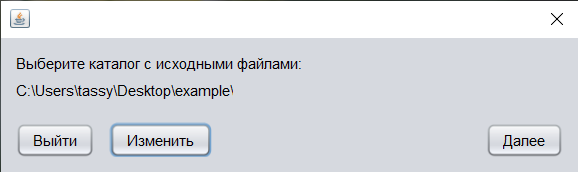
\includegraphics[width=0.7\linewidth]{pics/dir}
	\caption{Окно выбора директории}
	\label{fig:dir}
\end{figure}

В окне представлены три кнопки: «Выйти», «Изменить» и «Далее». 

При нажатии на кнопку «Изменить», открывается диалоговое окно с выбором каталога (рисунок~\ref{fig:edit-dir}).
\begin{figure}[H]
	\centering
	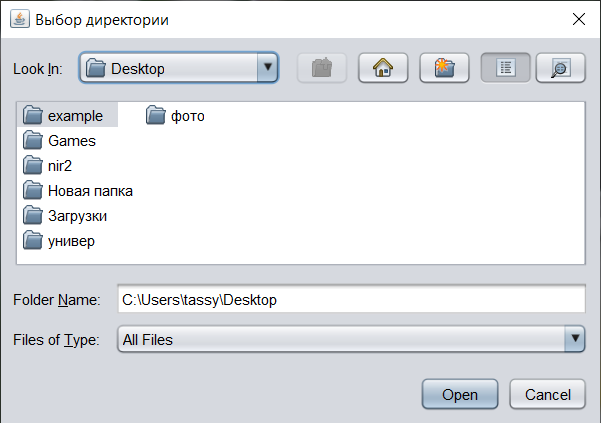
\includegraphics[width=0.7\linewidth]{pics/edit-dir}
	\caption{Диалоговое окно изменения директории}
	\label{fig:edit-dir}
\end{figure}

Указание директории при начале работы необходимо для корректной работы программы. Приложение использует данные из исходных файлов для отображения в пользовательском интерфейсе. В программе также предусмотрена возможность смены директории исходных файлов из главного меню.


\subsubsection{Главное меню}

После выбора исходной директории, при нажатии кнопки «Далее» происходит переход к окну с главным меню. 
\begin{figure}[H]
	\centering
	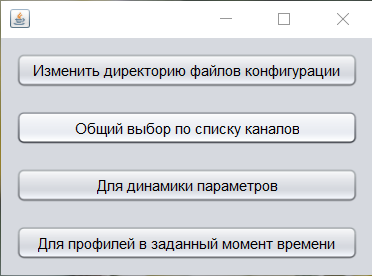
\includegraphics[width=0.7\linewidth]{pics/menu}
	\caption{Главное меню}
	\label{fig:menu}
\end{figure}

В главном меню собраны кнопки, отвечающие за основной функционал программы (рисунок~\ref{fig:menu}). Здесь присутствует кнопка «Изменить директорию файлов конфигурации». По своему функционалу она схожу с начальным окном выбора каталога. После неё идет группа из трёх кнопок, которые отвечают за задание параметров расчетных данных. В эту группу входят: выбор по списку каналов, выбор для динамики параметров и выбор для профилей в заданный момент времени. 

\subsubsection{Общий выбор по списку каналов}

Данное окно вызывается из окна с главным меню. В нём предоставляется возможность выбора канала, для которого нужно проводить визуализацию (рисунок~\ref{fig:chan}).
\begin{figure}[H]
	\centering
	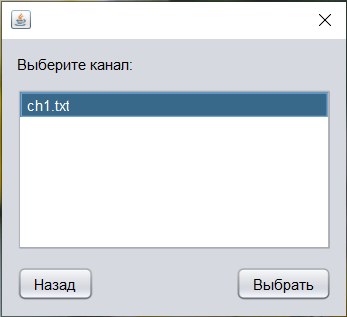
\includegraphics[width=0.4\linewidth]{pics/chan}
	\caption{Окно общего выбора по списку каналов}
	\label{fig:chan}
\end{figure}

В окне есть две кнопки: «Назад» и «Выбрать». Каналы выводятся в JList. JList используются для визуального отображения данных.  Выборка данных производится из файла, который содержит информацию о каналах (chanprof.txt). Загрузка и обработка данных совершается с помощью класса ChanProfReader. Он выполняет считывание и парсинг необходимых данных из файла конфигурации. 


\subsubsection{Выбор для динамики параметров}
Данное окно вызывается из окна с главным меню. В нём предоставляется возможность выбора координаты канала и переменных для отображения (рисунок~\ref{fig:dynam}).

\begin{figure}[H]
	\centering
	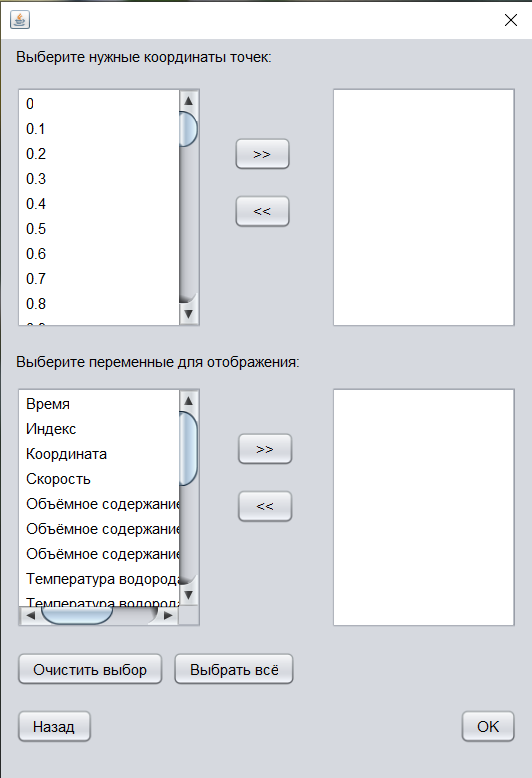
\includegraphics[width=0.5\linewidth]{pics/dynam}
	\caption{Окно выбора для динамики параметров}
	\label{fig:dynam}
\end{figure}

В окне представлены несколько списков, в которых отображаются доступные для выбора параметры и выбранные параметры (рисунок~\ref{fig:dynam-select}). Для осуществления выбора в окне есть несколько кнопок. Направление стрелок на кнопках соответствует направлению перемещения элементов из одного списка в другой. Также в окне присутствуют кнопки «Выбрать всё» и «Очистить список». Они реализуют упомянутые операции для элементов списка с параметрами наблюдений (рисунок~\ref{fig:dynam-all}). 
\begin{figure}[H]
	\centering
	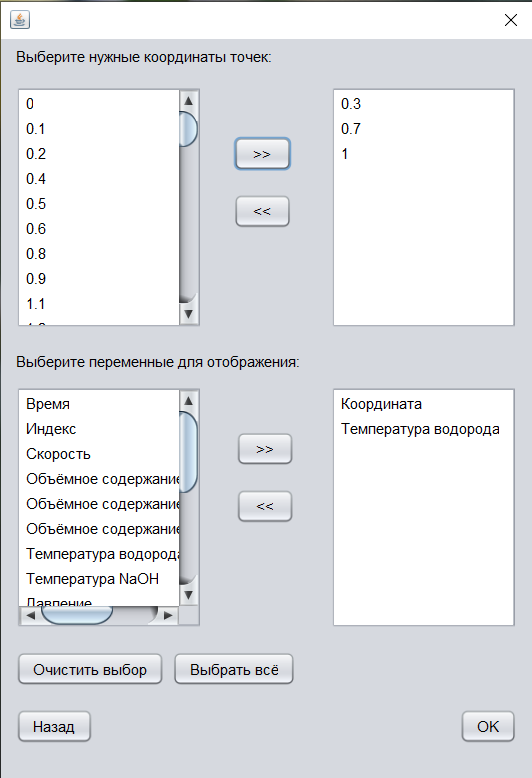
\includegraphics[width=0.5\linewidth]{pics/dynam-select}
	\caption{Окно выбора для динамики параметров}
	\label{fig:dynam-select}
\end{figure}

\begin{figure}[H]
	\centering
	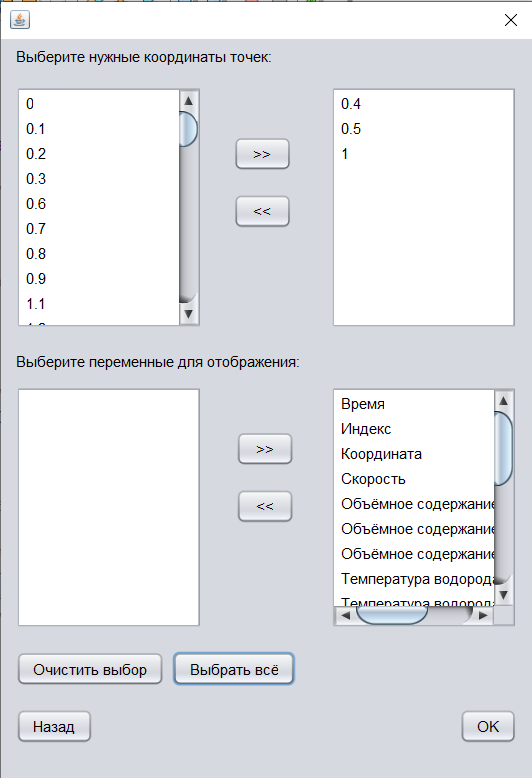
\includegraphics[width=0.5\linewidth]{pics/dynam-all}
	\caption{Окно выбора для динамики параметров}
	\label{fig:dynam-all}
\end{figure}

Выборка координат канала производится из файла с геометрий канала (geom.txt). Для этого производится подсчёт допустимых координат: исходя из шага сетки и длины канала, в цикле высчитываются все возможные координаты канала. Весь описанный функционал выполняется через класс GeomReader, который реализует считывание данных и их последующую обработку и необходимые вычисления. 

Выборка переменных для отображения производится из CSV-файла с метаданными по параметрам. Выполняется это с помощью класса CSVReader, который реализует считывание данных и их последующую обработку.

\subsubsection{Выбор для профилей в заданный момент времени}

Данное окно вызывается из окна с главным меню. В нём предоставляется возможность выбора момента времени моделирования и переменных для отображения (рисунок~\ref{fig:time}).

\begin{figure}[H]
	\centering
	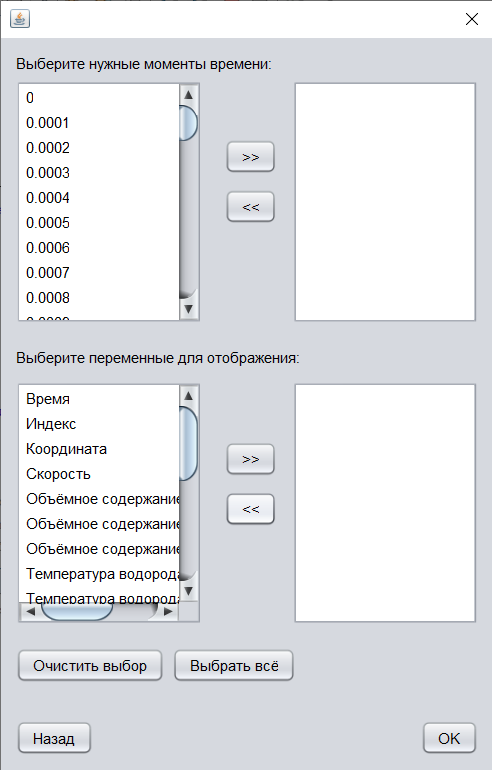
\includegraphics[width=0.5\linewidth]{pics/time}
	\caption{Окно выбора для профилей в заданный момент времени}
	\label{fig:time}
\end{figure}

В окне представлены несколько списков, в которых отображаются доступные для выбора параметры и выбранные параметры (рисунок~\ref{fig:time-select}). Для осуществления выбора в окне есть несколько кнопок. Направление стрелок на кнопках соответствует направлению перемещения элементов из одного списка в другой. Также в окне присутствуют кнопки «Выбрать всё» и «Очистить список». Они реализуют упомянутые операции для элементов списка с параметрами наблюдений (рисунок~\ref{fig:time-all}). 

\begin{figure}[H]
	\centering
	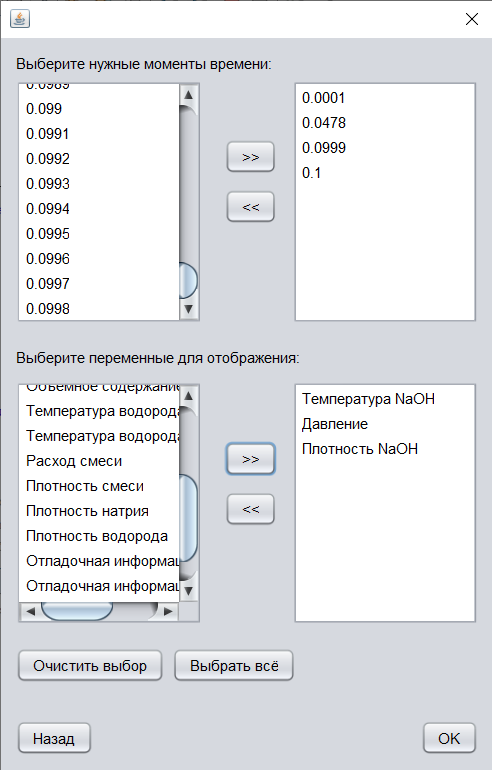
\includegraphics[width=0.5\linewidth]{pics/time-select}
	\caption{Окно выбора для профилей в заданный момент времени}
	\label{fig:time-select}
\end{figure}

\begin{figure}[H]
	\centering
	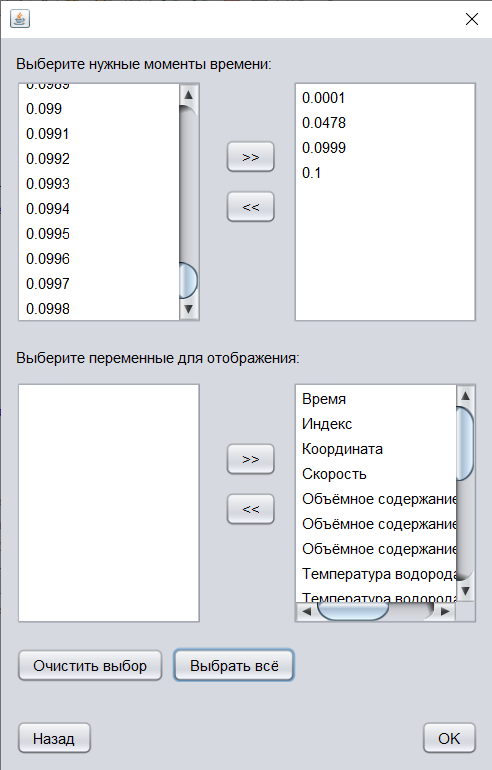
\includegraphics[width=0.5\linewidth]{pics/time-all}
	\caption{Окно выбора для профилей в заданный момент времени}
	\label{fig:time-all}
\end{figure}
Выборка моментов времени производится из файла со сценарием сохранения результатов (timescen.txt). Для этого производится подсчёт допустимых моментов времени: исходя из количества временных интервалов моделирования и шага интервалов, в цикле высчитываются все возможные временные моменты. Весь описанный функционал выполняется через класс TimeReader, который реализует считывание данных и их последующую обработку и необходимые вычисления. 

Выборка переменных для отображения производится так же, как и в окне выбора для динамики параметров. 

  % третья глава - в файле part3.tex
\pagebreak

% если есть еще разделы - сохраните их в соответствующих файлах и раскомментируйте строки ниже, при необходимости добавьте еще
%\input{part4} % четвертая глава - в файле part4.tex
%\pagebreak

%\input{part5}  % пятая глава - в файле part5.tex
%\pagebreak

\section*{\centering ЗАКЛЮЧЕНИЕ}
\addcontentsline{toc}{section}{ЗАКЛЮЧЕНИЕ}

В результате выполнения научно-исследовательской  работы были решены следующие задачи:

\begin{itemize}
\item выполнен анализ структуры конфигурационных и расчётных файлов;
\item разработаны вспомогательные классы для считывания конфигурации;
\item разработаны классы, описывабщие структуру расчетных файлов;
\item спроектирован и разработан пользовательский интерфейс задания параметров расчётных данных.

\end{itemize}


\pagebreak
% оформление библиографии - вариант с БД
\addcontentsline{toc}{section}{СПИСОК ИСПОЛЬЗОВАННЫХ ИСТОЧНИКОВ}
% ВАЖНО: для корректного отображения в списке литературы ссылок на англ.языке в bibtex-описание источника следует добавить поле 
% langid = {english}
\printbibliography


%\pagebreak

\renewcommand{\appendixpagename}{\centering Приложения}


\begin{appendices}
\renewcommand{\thesection}{\Asbuk{section}}
\makeatletter
\renewcommand{\theProgram}{\thesection.\@arabic\c@Program}
\renewcommand{\thefigure}{\thesection.\@arabic\c@figure}
\makeatother

% каждое приложение задается следующей командой, нумерация - русскими буквами
\section{\centering } 
% независимая нумерация листингов в каждом приложении
\setcounter{Program}{0}
\setcounter{figure}{0}

\begin{MyCode}[fontsize=\small]

public class DefaultReader {
	protected ArrayList<String> fileInf = null;
	
	
	public void readFile (String path) {
		java.io.FileReader fr = null;
		ArrayList<String> arr = new ArrayList<>();
		try {
			
			fr = new java.io.FileReader(path);
			Scanner scan = new Scanner(fr);
			String s;
			
			while (scan.hasNextLine()) {
				s = scan.nextLine();
				arr.add(s);
				
			}
		} catch (FileNotFoundException ex) {
			Logger.getLogger(Lleak.class.getName()).log(Level.SEVERE, null, ex);
		} 
		finally {
			if (fr != null) {
				try {
					fr.close();
				} catch (IOException ex) {
					Logger.getLogger(Lleak.class.getName()).log(Level.SEVERE, null, ex);
				}
				
			}
		}
		
		fileInf = arr;  
		
	}
	
	protected DefaultReader() {
	}
	
	public ArrayList<String> getFileInf() {
		return fileInf;
	}     
}

\end{MyCode}
\nopagebreak
\begin{Program}
	\caption{Суперкласс DefaultReader}\label{DefReader}
\end{Program}

\pagebreak




\end{appendices}


\end{document}          


% следующее приложение - раскомментировать команды
%\section{\centering } 
%\setcounter{Program}{0}
%\begin{MyCode}
%код третьего приложения
%\end{MyCode}
%\nopagebreak
%\begin{Program}
%\caption{Еще пример кода}\label{app3}
%\end{Program}

